\section{Erläuterung der einheitlichen Speicherlösung}\label{konzeption_ssot}

\tikzstyle{block} = [draw, fill=white!20, rectangle, 
    minimum height=3em, minimum width=6em]
\tikzstyle{sum} = [draw, fill=blue!20, circle, node distance=2cm]
\tikzstyle{input} = [coordinate]
\tikzstyle{output} = [coordinate]
\usetikzlibrary{arrows.meta,arrows}

Die Interviews des Kapitels \ref{anforderungsanalyse} ergaben, dass eine neue Plattform gewünscht wird, bei der das Wechseln zwischen verschiedenen visuellen Repräsentationen der Roboter möglich ist. Dadurch können sowohl Low-Code-Developer als auch professionelle Entwickler in ihrer präferierten Umgebung Automatisierungen erstellen.

Nachfolgend wird erläutert, mit welcher Architektur sich diese Funktionalität implementieren lässt und warum hierfür eine einheitliche Speicherlösung (Single Source of Truth) benötigt wird. Im Anschluss werden die Anforderungen an die SSoT dargestellt.

\subsection{Konzeption der Architektur}

Um die visuelle Repräsentation eines Roboters in den ausführbaren Code der RobotFramework Syntax zu übersetzen, werden die eingangs beschriebenen Parser benötigt. Sofern ausschließlich Robotermodelle in ausführbaren Code übersetzt werden sollen und somit kein Wechsel der Modellierungssprache bei der Erstellung eines Roboters möglich ist, genügt die in Abbildung \ref{fig:parser1} gezeigte Architektur. Hierbei wird für jeden Roboter die visuelle Repräsentation um die benötigten RPA-Eigenschaften angereichert und gespeichert. Im Beispiel von \code{bpmn-js} ist das Speicherformat ein XML, in dem jede BPMN-Aktivität um die Tags \code{<rpaApplication>} und \code{<rpaTask>} erweitert werden kann. Soll nun der Roboter ausgeführt werden, wird die aktuelle Version des XML-Files in den ausführbaren Code geparst. Dadurch wird für jedes unterstützte Interface genau ein Parser benötigt.

\begin{figure}[h!]
    \centering
    \begin{tikzpicture}[auto, show background rectangle, node distance=2cm,>=latex']
        \node [block, name= robot] (robot) {.ROBOT};
        \node [block, above left= 0.5cm and -0.5cm of robot, name=pap] {PAP};
        \node [block, above right= 0.5cm and -0.5cm of robot, name=epk] {EPK};
        \node [block, left=1cm of pap] (bpmn) {BPMN};
        \node [block, right=1cm of epk] (other) {...};
        \draw [-{Stealth[scale=2]}] (bpmn.south) -- (robot.west);
        \draw [-{Stealth[scale=2]}] (pap.south) -- (robot);
        \draw [-{Stealth[scale=2]}] (epk.south) -- (robot);
        \draw [-{Stealth[scale=2]}] (other.south) -- (robot.east);
    \end{tikzpicture}
    \caption{Lokation der Parser ohne Wechsel zwischen den Darstellungsformen}
    \label{fig:parser1}
\end{figure}

\clearpage

Um denselben Roboter in verschiedenen Notationen erstellen zu können, bedarf es in einer trivialen Lösung zwischen jedem Paar von Interfaces zweier Parser. Diese Variante der Implementierung ist in der Abbildung \ref{fig:parser2} dargestellt. Bei dieser und der nachfolgenden Lösung ist es zudem möglich, direkt in dem auszuführenden Code Änderungen vorzunehmen und diese im Anschluss auch in den Notationen zu sehen. Problematisch ist jedoch, dass bei dieser Architektur exponentiell viele Parser in Abhängigkeit der angebotenen Interfaces benötigt werden. Zudem müsste sich auf eine Repräsentation geeinigt werden, in der der Roboter persistent gespeichert wird. 

\begin{figure}[h!]
    \centering
    \begin{tikzpicture}[auto,show background rectangle, node distance=2cm,>=latex']
        \node [block, name= robot] (robot) {.ROBOT};
        \node [block, above left= 0.5cm and -0.5cm of robot, name=pap] {PAP};
        \node [block, above right= 0.5cm and -0.5cm of robot, name=epk] {EPK};
        \node [block, left=1cm of pap] (bpmn) {BPMN};
        \node [block, right=1cm of epk] (other) {...};
        \draw [{Stealth[scale=2]}-{Stealth[scale=2]}] (bpmn.south) -- (robot.west);
        \draw [{Stealth[scale=2]}-{Stealth[scale=2]}] (pap.south) -- (robot);
        \draw [{Stealth[scale=2]}-{Stealth[scale=2]}] (epk.south) -- (robot);
        \draw [{Stealth[scale=2]}-{Stealth[scale=2]}] (bpmn) -- (pap);
        \draw [{Stealth[scale=2]}-{Stealth[scale=2]}] (pap) -- (epk);
        \draw [{Stealth[scale=2]}-{Stealth[scale=2]}] (other.south) -- (robot.east);
        \draw [{Stealth[scale=2]}-{Stealth[scale=2]}] (other) -- (epk);
        \draw [{Stealth[scale=2]}-{Stealth[scale=2]}] (bpmn) to [out=25,in=155] (epk.north);
        \draw [{Stealth[scale=2]}-{Stealth[scale=2]}] (pap.north) to [out=25,in=155] (other);
        \draw [{Stealth[scale=2]}-{Stealth[scale=2]}] (bpmn.north) to [out=20,in=160] (other.north);
    \end{tikzpicture}
    \caption{Lokation der Parser ohne einheitliche Datenspeicherlösung}
    \label{fig:parser2}
\end{figure}

Um nur linear viele Parser zu benötigen, stellt diese Arbeit eine Architektur vor, die auf einer Single Source of Truth basiert. Diese SSoT dient als einheitliches Speicherformat der Roboter. Aus ihr werden alle visuellen Repräsentationen erstellt und ebenso resultieren alle Änderungen in den grafischen Editoren in der SSoT. Zur Realisierung dieses Konzeptes werden pro Notation zwei Parser benötigt (\mbox{Abbildung \ref{fig:parser3}).}

\begin{figure}[h!]
    \centering
    \begin{tikzpicture}[auto,show background rectangle, node distance=2cm,>=latex']
        \node [block, fill=black!30!green, rounded corners=0.5cm] (ssot) {SSoT};
        \node [block, above left= 0.7cm and 1.2cm of ssot, name=pap] {PAP};
        \node [block, above right= 0.7cm and 1.2cm of ssot, name=epk] {EPK};
        \node [block, left=2.65cm of ssot] (bpmn) {BPMN};
        \node [block, right=2.65cm of ssot] (other) {...};
        \node [block, above=0.7cm of ssot] (robot) {.ROBOT};
        \draw [{Stealth[scale=2]}-{Stealth[scale=2]}] (ssot) -- (robot);
        \draw [{Stealth[scale=2]}-{Stealth[scale=2]}] (ssot) -- (bpmn);
        \draw [{Stealth[scale=2]}-{Stealth[scale=2]}] (ssot) -- (epk.south);
        \draw [{Stealth[scale=2]}-{Stealth[scale=2]}] (ssot) -- (pap.south);
        \draw [{Stealth[scale=2]}-{Stealth[scale=2]}] (ssot) -- (other);
    \end{tikzpicture}
    \caption{Lokation der Parser mit einheitlicher Datenspeicherlösung}
    \label{fig:parser3}
\end{figure}

\clearpage

\subsection{Konzeption der Speicherlösung}

Betrachten wir nun das Konzept hinter der einheitlichen Speicherlösung. Diese Datenstruktur speichert alle relevanten Daten des Roboters, sodass daraus der finale Ausführungscode sowie alle visuellen Repräsentationen erstellt (engl. „geparst“) werden können.

Ziel der Speicherlösung ist es, die visuellen Repräsentationen zu abstrahieren und nur die Semantik zu speichern. Dafür wird für jede Modellierungssprache die ihr zugrunde liegende Programmierlogik abgeleitet und nur diese gespeichert. 
Für die Programmierkonzepte werden nachfolgend Typen definiert, mit deren Hilfe sich alle Graphen abspeichern lassen (siehe Tabelle \ref{tab:ssot-types}). Zusätzlich ist der Typ „\code{MARKER}“ definiert, der entweder Start oder Ende des Roboters beschreibt. Dadurch wird ermöglicht, die Start- und Endsymbole der BPMN, Flowcharts und EPKs - wie im Standard gewünscht - zu benennen. 

\begin{table}[h!]
    \caption{Typen der Single Source of Truth}
    \centering
        \begin{tabular}{|l|l|}
        \hline
        \textbf{Programming Construct} & \textbf{SSoT-Type} \\ \hline
        Single Statement               & INSTRUCTION       \\ \hline
        Branching                      & CASE              \\ \hline
        Loop                           & LOOP              \\ \hline
        Start / End of Robot           & MARKER            \\ \hline
        \end{tabular}
    \label{tab:ssot-types}
\end{table}

Die SSoT besteht aus einem Header, der die Meta-Informationen des Roboters wie die \code{RobotId}, den Namen des Roboters und die Id des ersten Knotens im Graphen speichert. Darauf folgt das \code{ElementArray}, das alle Programmteile des Roboters enthält.  Jedes Element des Element-Arrays besitzt ein Feld zur Angabe des Typs (\code{INSTRUCTION}, \code{CASE}, \code{LOOP} o. \code{MARKER}). Zudem wird für jedes Element der Name, eine Id, die Id der Vorgänger- und Nachfolger im Grahpen  sowie optional ein Dokumentationstext gespeichert. 

Wie in Abbildung \ref{fig:aufbauSSOT} zu sehen, kann jedes Element in Abhängigkeit des Typs um weitere Felder angereichert werden. Dazu zählen beispielsweise bei einer Anweisung (\code{INSTRUCTION}) die benötigten Informationen des RPA-Statements. Das Schleifen-Element (\code{LOOP}) speichert neben der Schleifenabbruchbedingung die Id’s der Anfangs- und Endknoten des Schleifenkörpers, um eine vollständige Rekonstruktion des Graphens zu ermöglichen. \code{MARKER} benötigen keine weiteren Attribute.

\begin{figure}[h!]
    \centering
    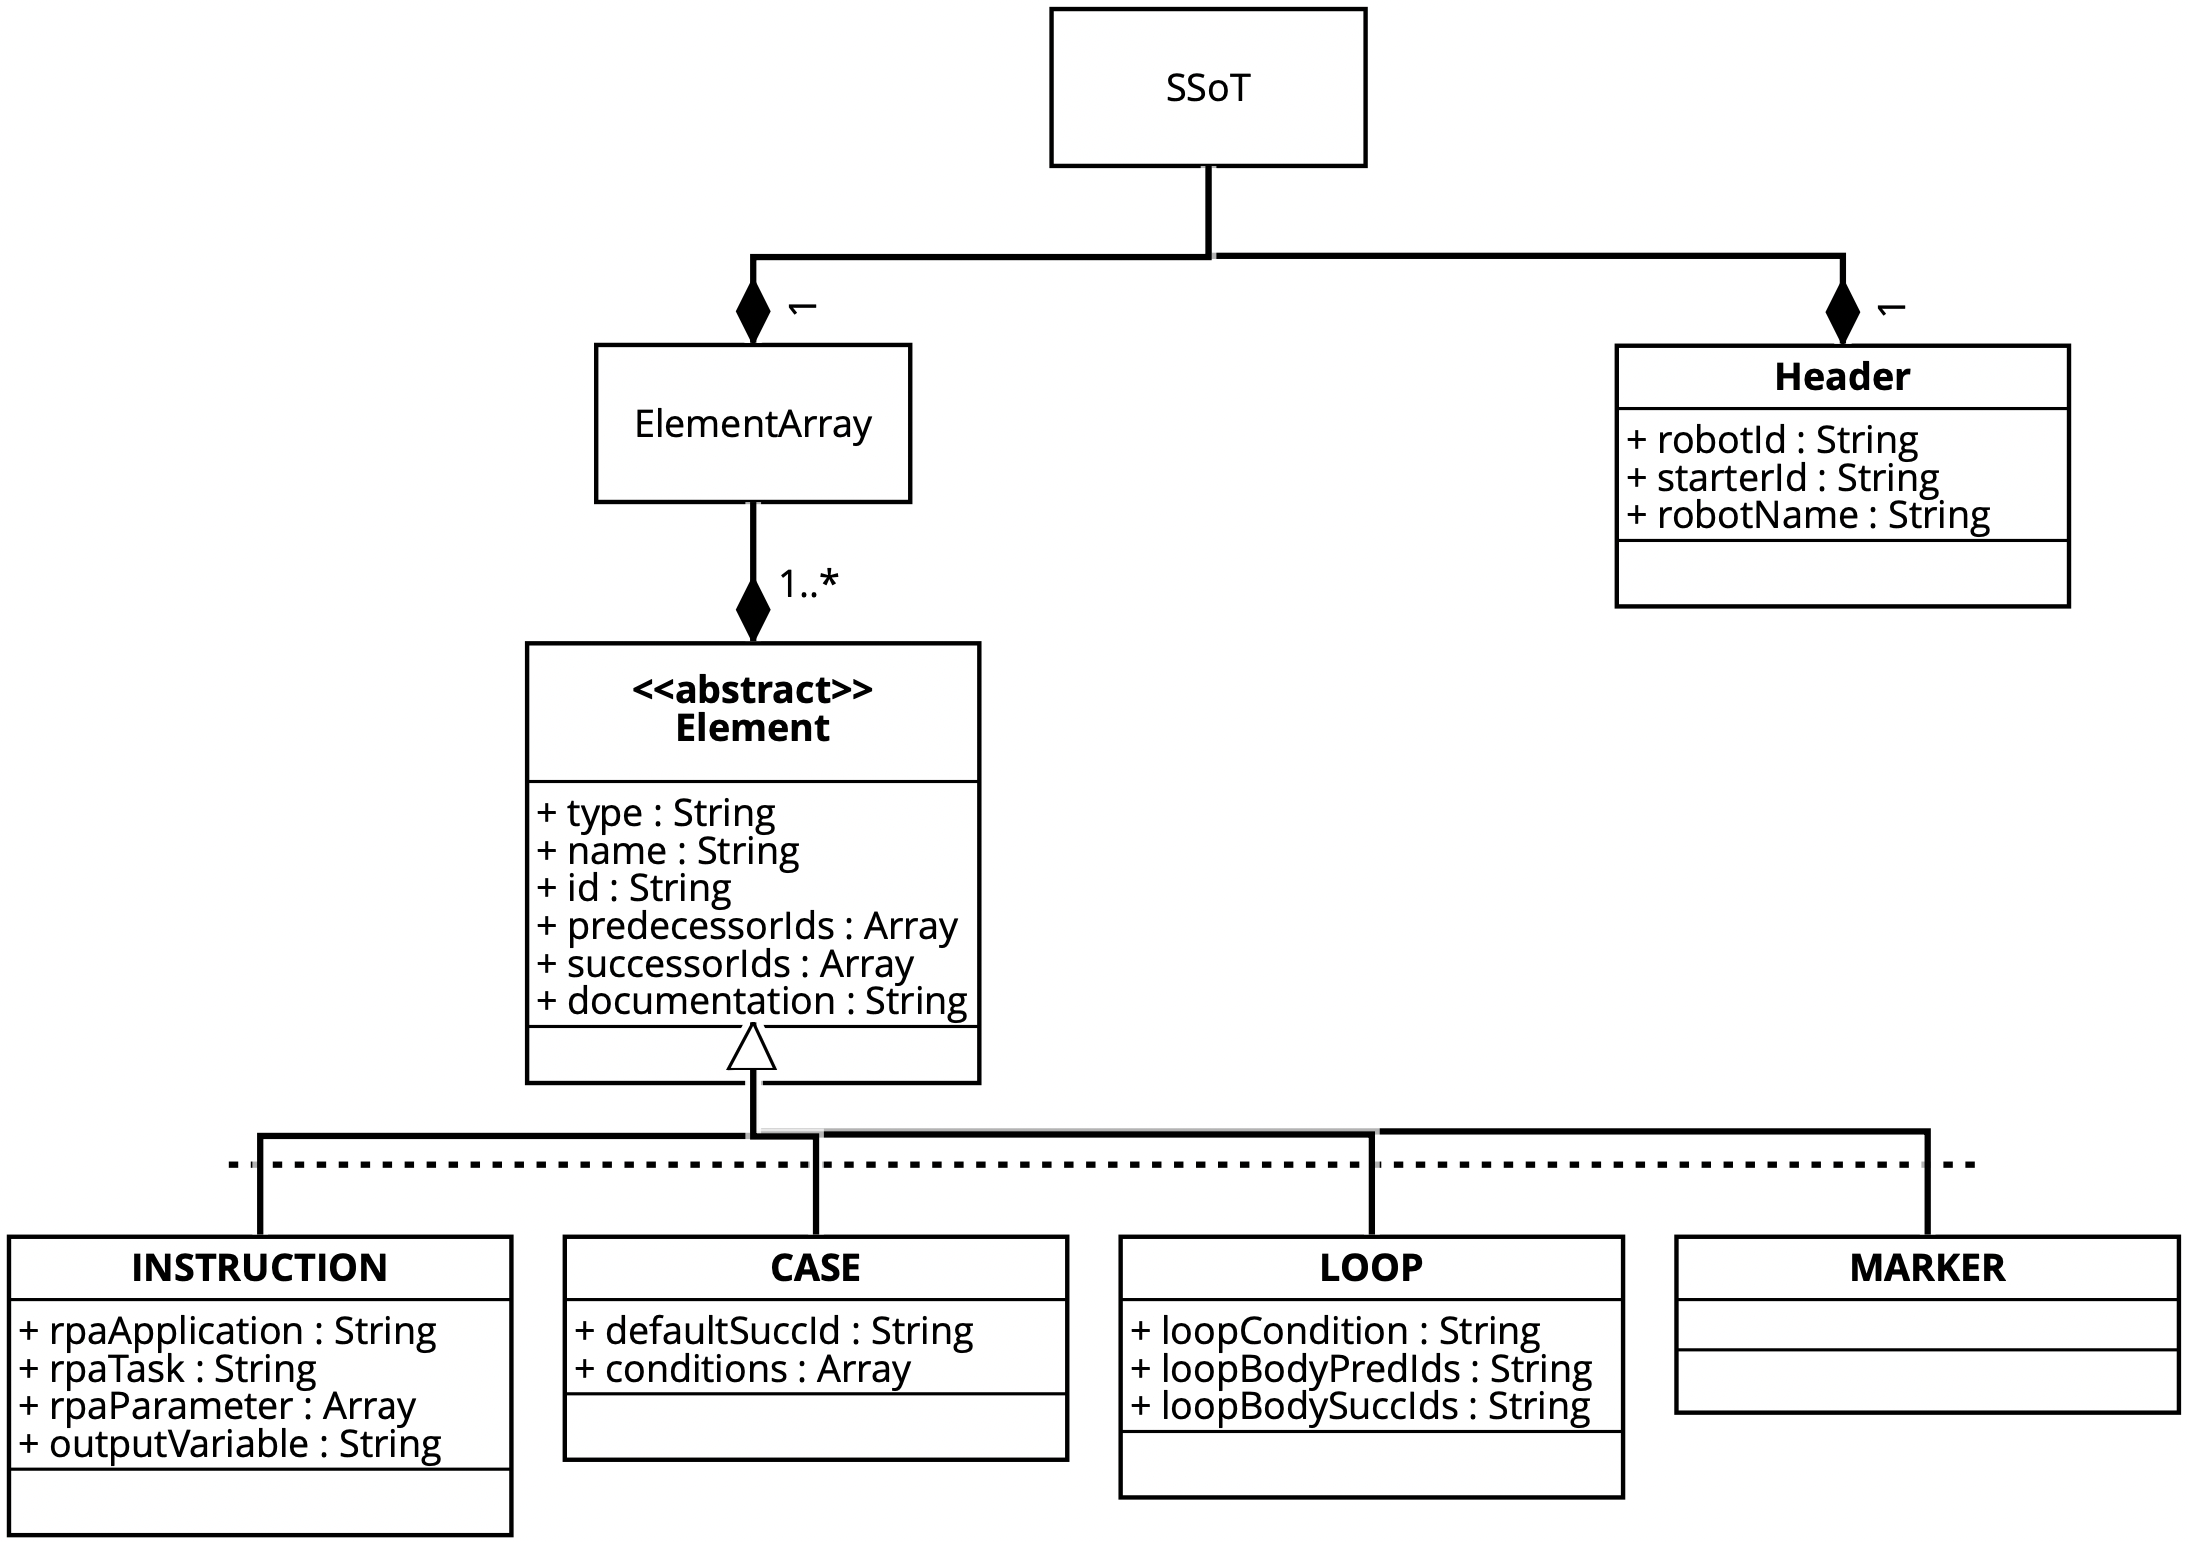
\includegraphics[width=1\textwidth]{Bachelorarbeit/images/aufbauSSOT2.png}
    \caption{Hierarchischer Aufbau der Datenspeicherlösung}
    \label{fig:aufbauSSOT}
\end{figure}

Der den Roboter beschreibende Graph lässt sich mit den Informationen zu Vorgänger- und Nachfolgerknoten eindeutig zusammensetzen. Somit kann aus der SSoT jede visuelle Repräsentation rekonstruiert werden. Es werden keine spezifischen Eigenschaften der Modellierungssprachen, wie zum Beispiel die absolute Position eines Knotens gespeichert. Daher müssen diese Werte auf Grundlage des Graphens errechnet werden, wodurch die Modelle sich bei jedem erneuten Rendering automatisch ausrichten und formatieren.

Die meisten Felder der Elemente werden mit Strings befüllt. Eine Besonderheit ist hierbei das \code{rpaParameter}-Array des \code{INSTRUCTION}-Elements. In diesem Array werden benötigte Eingabeparameter für die ausgewählte \code{rpaApplication/rpaTask}-Kombination angegeben. Somit kann dieses Array auch leer sein, sofern der Funktionsaufruf keine Parameter benötigt. 

\label{parameterProps}
Jeder Parameter repräsentiert wiederum ein Objekt, in dem der Name des Parameters, ein Hinweistext, eine boolesche Variable (die aussagt, ob der Parameter zwingend angegeben werden muss), sowie die Position des Parameters aus der RpaFramework-Dokumentation angegeben wird. Diese Ganzzahl gibt in Zusammenhang mit den anderen Parametern an, in welcher Ordnung die Parameter in den auszuführenden Code zu parsen sind.
Zudem werden für jeden Parameter der Typ wie beispielsweise \code{String} oder \code{Integer} sowie dessen Wert gespeichert.